\section{Introduzione alla Gestione delle Identità e degli Accessi}
La gestione delle identità e degli accessi (IAM) rappresenta un passo fondamentale per sviluppare qualsiasi strategia di sicurezza robusta in un ambiente cloud come Amazon Web Services (AWS). Per una startup fintech, dove la struttura gerarchica è ancora poco definita, stabilire chi può accedere alle risorse e con quali privilegi non è solo una best practice, ma una necessità imprescindibile per garantire una gestione sicura e affidabile dei dati. Questo capitolo esplora i principi cardine della sicurezza IAM, analizza la configurazione attuale della startup "Finanz" e propone una serie di miglioramenti concreti per rafforzare la postura di sicurezza, ispirandosi ai modelli Zero Trust e al Principio del Minimo Privilegio. L'obiettivo è creare un framework IAM che sia non solo sicuro, ma anche flessibile e gestibile, per supportare la crescita dinamica della startup.



\subsection{Configurazione dell'infrastruttura AWS per la piattaforma \textit{Finanz}}
\label{subsec:aws_infrastruttura_attuale_cap4_narrativo}

\paragraph{Panoramica architetturale}
L'infrastruttura tecnologica che supporta la piattaforma \textit{Finanz} è interamente provisionata all'interno della regione AWS `eu-south-1` (Milano) e consolidata in un singolo account. Per garantire una netta separazione degli ambienti, sono stati definiti due contesti logici distinti, `Finanz-Dev` per lo sviluppo e `Finanz-Prod` per la produzione. La segregazione tra questi non avviene a livello di account, bensì è implementata attraverso una strategia granulare di tagging delle risorse, l'impiego di ruoli IAM (Identity and Access Management) con permessi specifici e l'adozione di pipeline di rilascio completamente separate e indipendenti.

\paragraph{Layer applicativo}
Il layer applicativo, che ospita il servizio core `Finanz-Backend`, è orchestrato tramite il servizio gestito \textbf{AWS Elastic Beanstalk}. Tale servizio astrae la gestione dell'infrastruttura sottostante, automatizzando il provisioning e la configurazione delle risorse. La configurazione prevede l'impiego di istanze EC2 di tipo *burstable* (`t3a.small`), definite tramite un Launch Template. La scalabilità orizzontale è gestita da un Auto Scaling Group, le cui politiche sono basate su metriche di carico della CPU e sul numero di richieste al secondo, con soglie differenziate tra l'ambiente di sviluppo (da 1 a 2 istanze) e quello di produzione (da 3 a 5 istanze). Un Application Load Balancer (ALB) funge da unico entry-point per il traffico HTTPS, instradandolo verso le istanze applicative. Queste ultime sono protette da un Security Group che ne permette l'accesso esclusivamente dall'ALB, isolandole da accessi diretti. Infine, i log applicativi e di sistema vengono inoltrati in tempo reale verso Amazon CloudWatch Logs per il monitoraggio e archiviati su Amazon S3 con rotazione oraria per l'analisi a lungo termine.

\paragraph{Layer dati}
Il layer di persistenza dei dati transazionali si affida al servizio gestito \textbf{Amazon RDS for PostgreSQL}. La sicurezza dei dati *at-rest* è garantita dalla cifratura, attuata tramite una chiave gestita dal cliente (Customer-Managed Key) in AWS Key Management Service (KMS). Per rispondere a diverse esigenze di disponibilità e costo, l'ambiente di produzione impiega un'istanza in configurazione Multi-AZ, che assicura alta disponibilità e failover automatico, con una retention dei backup di sette giorni e la protezione contro la cancellazione accidentale. Al contrario, l'ambiente di sviluppo utilizza un'istanza Single-AZ, con backup disabilitati. Per entrambe le configurazioni, l'accesso pubblico è negato e i log di database, insieme alle metriche di Performance Insights, vengono aggregati in Amazon CloudWatch per un monitoraggio centralizzato delle prestazioni.

\paragraph{Topologia di rete}
La rete è incapsulata in un Virtual Private Cloud (VPC) con un ampio spazio di indirizzamento privato (`10.0.0.0/16`). La segmentazione è ottenuta attraverso una topologia multi-tier che prevede subnet pubbliche e private. Una subnet pubblica ospita le risorse che necessitano di esposizione diretta a Internet, ovvero l'Application Load Balancer e un NAT Gateway. Le risorse computazionali, cioè le istanze EC2, risiedono invece in subnet private dedicate, una per l'ambiente di produzione e una per quello di sviluppo. Questo disegno architetturale assicura che le istanze applicative non siano mai direttamente raggiungibili dall'esterno. Il traffico in ingresso (\textbf{ingress}) è sempre mediato dall'ALB, mentre il traffico in uscita (\textbf{egress}), necessario per le chiamate a servizi esterni, è canalizzato attraverso il NAT Gateway. Le tabelle di rotta sono configurate di conseguenza, impedendo alle subnet private qualsiasi rotta diretta verso l'Internet Gateway.

\paragraph{Storage e processi CI/CD}
Per lo storage degli artefatti e dei log si utilizzano bucket Amazon S3, protetti da policy restrittive. Il bucket impiegato da Elastic Beanstalk per le versioni applicative è protetto contro la cancellazione accidentale, mentre quello associato ad \textbf{AWS CodePipeline}, che contiene gli artefatti di build, impone la cifratura lato server e la comunicazione tramite TLS. Il processo di Continuous Delivery è automatizzato da una pipeline in CodePipeline, articolata nelle fasi canoniche di Source, Build e Deploy. La fase di Source è innescata da commit su branch specifici per lo sviluppo e da tag semantici per la produzione. La fase di Build, eseguita da \textbf{AWS CodeBuild}, include passaggi di sicurezza aggiuntivi per l'ambiente produttivo, come l'analisi di vulnerabilità (SCA/CVE) e la firma digitale degli artefatti. Infine, la fase di Deploy avviene con una strategia di *rolling update* per minimizzare i disservizi, e richiede un'approvazione manuale per ogni rilascio in produzione. Gli eventi salienti della pipeline vengono notificati tramite Amazon SNS.


\begin{figure}[htbp]
  \centering
  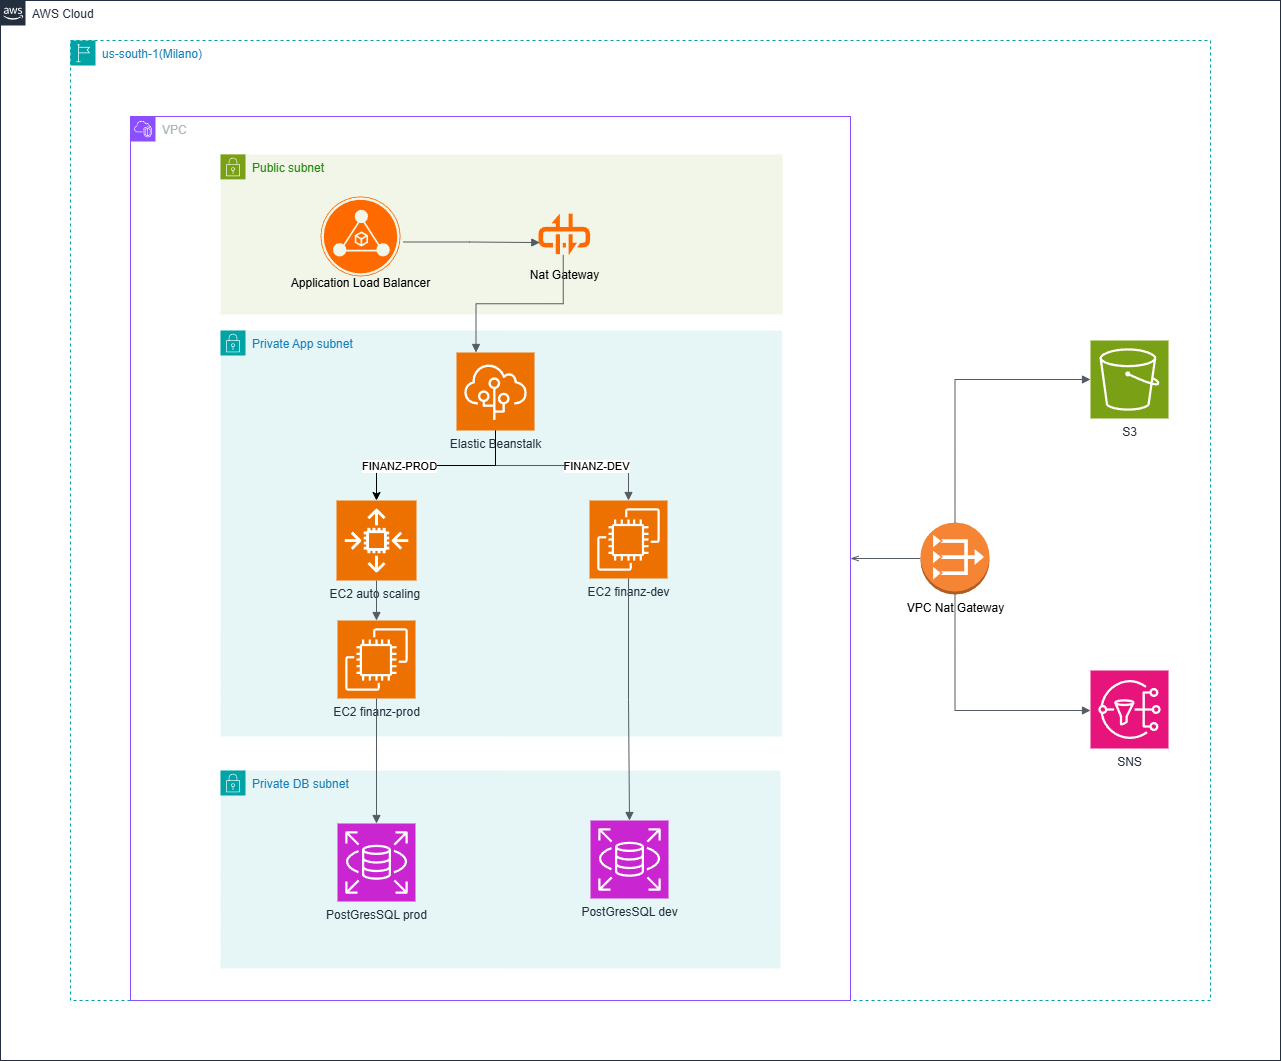
\includegraphics[width=0.8\textwidth]{aws_struttura}
  \caption{Diagramma semplificato dell’architettura AWS di \textit{Finanz}.}
  \label{fig:aws_struttura_attuale_cap2}
\end{figure}


\subsection{Implementazione del Modello Zero Trust e del Principio del Minimo Privilegio}
\label{sec:zero-trust-implementation}

Come già analizzato [\ref{ch:principi-cybersecurity}], il modello \textbf{Zero Trust} rappresenta un superamento del paradigma di sicurezza tradizionale basato sul perimetro. L'adozione di questo principio risulta cruciale nel contesto delle startup, i cui ambienti operativi sono per natura dinamici e flessibili. Le caratteristiche intrinseche delle startup non solo giustificano, ma impongono la necessità di un framework di sicurezza ispirato a tale modello. Approfondiamo ora gli aspetti chiave a sostegno di questa visione:

\begin{itemize}
  \item \textbf{Instabilità relazionale:} Le relazioni professionali nelle startup possono deteriorarsi rapidamente a causa della pressione elevata, degli obiettivi spesso poco definiti e della mancanza di esperienza nella gestione dei conflitti, sia a livello dirigenziale che operativo. Questi fattori creano tensioni che possono sfociare in incomprensioni e scontri personali. Secondo un'analisi di CB Insights, i conflitti interni tra fondatori rappresentano una delle principali cause di fallimento delle startup, incidendo per circa il 13\% dei casi esaminati \cite{CBInsights2023}.
  \item \textbf{Rischio di attacchi interni:} La fragilità dei rapporti interni, unita a dinamiche di potere e insoddisfazioni personali, aumenta la probabilità che ex-collaboratori con accessi privilegiati possano compiere azioni vendicative o dannose. Questo rischio è amplificato dalla scarsa attenzione alle politiche di controllo degli accessi e alla gestione delle risorse umane. Il "2023 Data Breach Investigations Report" di Verizon evidenzia che circa il 20\% delle violazioni di dati coinvolge insider, sottolineando l’importanza di monitorare e limitare gli accessi privilegiati \cite{Verizon2023}.
  \item \textbf{Infrastrutture di sicurezza inadeguate:} Le startup spesso destinano la maggior parte delle risorse allo sviluppo del prodotto e alla crescita del mercato, trascurando gli investimenti in infrastrutture di sicurezza. Inoltre, la mancanza di personale specializzato e di processi consolidati rende difficile implementare misure efficaci. Un rapporto del Ponemon Institute mostra che le piccole organizzazioni hanno una probabilità tre volte maggiore di subire attacchi informatici rispetto alle grandi imprese, proprio a causa di investimenti insufficienti e di una cultura della sicurezza ancora poco sviluppata \cite{Ponemon2023}.
\end{itemize}
Questa sezione illustra come i principi Zero Trust possano essere tradotti in misure di sicurezza concrete all'interno dell'infrastruttura cloud di una startup, con specifico riferimento all'ambiente AWS. Ci concentreremo in particolare sulla gestione delle identità e degli accessi, un pilastro fondamentale per qualsiasi architettura Zero Trust, e sulla sua stretta interconnessione con il \textbf{Principio del Minimo Privilegio (Principle of Least Privilege - PoLP)}.
\subsubsection{Sinergia tra Principio del Minimo Privilegio (PoLP) e Zero Trust}
\label{subsubsec:polp-zerotrust-correlation}

Il Principio del Minimo Privilegio non è solo una buona pratica di sicurezza a sé stante, ma è intrinsecamente legato e \textbf{fondamentale per il successo di un'architettura Zero Trust}. La loro sinergia si manifesta in diversi modi:

\begin{itemize}
    \item \textbf{Riduzione della Superficie d'Attacco:} Limitando strettamente le azioni consentite a ciascuna identità, PoLP riduce l'insieme delle operazioni che un attaccante potrebbe eseguire anche riuscendo a compromettere le credenziali di quell'identità. La verifica dell'identità (Zero Trust) è necessaria ma non sufficiente; i privilegi limitati (PoLP) ne circoscrivono le capacità.
    \item \textbf{Limitazione del Raggio d'Esplosione (\textit{Blast Radius})}: In caso di compromissione o errore, i danni potenziali sono confinati. Un utente o servizio con privilegi minimi non può accedere o modificare risorse al di fuori del suo ambito operativo ristretto, limitando il movimento laterale dell'attaccante e l'impatto dell'incidente.
    \item \textbf{Applicazione della Verifica Esplicita:} Implementare PoLP costringe a definire policy di accesso granulari e intenzionali, basate sulle reali necessità operative. Questo si allinea perfettamente con la richiesta di Zero Trust di basare ogni decisione di accesso su policy esplicite e dinamiche, piuttosto che su autorizzazioni ampie o ereditate implicitamente.
    \item \textbf{Miglioramento del Controllo e dell'Auditabilità:} Policy di accesso minimali e specifiche sono più facili da comprendere, gestire e verificare. Ciò semplifica l'audit della postura di sicurezza e la dimostrazione della conformità, permettendo di attestare che gli accessi sono effettivamente limitati come richiesto dal modello Zero Trust.
\end{itemize}
\subsection{Gestione delle Identità e degli Accessi (IAM) come Pilastro di Zero Trust in AWS}
\label{subsec:iam-zero-trust}

L'infrastruttura ospitata su un Cloud Service Provider (CSP) come AWS è un asset critico per una startup fintech. Essa contiene dati sensibili degli utenti e ospita i servizi essenziali (endpoint API, istanze EC2 per server applicativi, networking VPC, ecc.) che ne garantiscono l'operatività. La protezione di queste risorse inizia dalla gestione rigorosa di chi può accedervi e cosa può fare. \textbf{AWS Identity and Access Management (IAM)} è il servizio centrale per implementare questi controlli e costituisce una base imprescindibile per un modello Zero Trust.

Una delle prime e più critiche aree di intervento riguarda l'\textbf{account root di AWS}. Questo account possiede privilegi illimitati sull'intero ambiente AWS e rappresenta, di conseguenza, un obiettivo di altissimo valore per gli attaccanti e una fonte significativa di rischio operativo se usato impropriamente. Un'implementazione Zero Trust richiede misure stringenti per l'account root:
\begin{itemize}
    \item \textbf{Limitazione Estrema dell'Uso:} L'accesso come utente root deve essere evitato per le operazioni quotidiane e riservato esclusivamente a quelle poche attività che lo richiedono obbligatoriamente (es. modifica delle informazioni di fatturazione, chiusura dell'account, modifica dei piani di supporto).
    \item \textbf{Protezione Robusta delle Credenziali:} La password deve essere estremamente complessa e, soprattutto, l'\textbf{Auten\-ticazione a Più Fattori (MFA)} deve essere \textit{sempre} abilitata e richiesta per l'accesso root.
    \item \textbf{Monitoraggio Continuo:} Ogni azione eseguita tramite l'account root deve essere tracciata e monitorata tramite servizi come AWS CloudTrail, generando allarmi per qualsiasi utilizzo.
\end{itemize}


\subsection{Valutazione dell'implementazione IAM corrente di \emph{Finanz}}
\label{subsec:analisi_iam_finanz}

\subsubsection*{Analisi degli accessi e delle policy}
L'analisi dell'infrastruttura di \emph{Finanz} (marzo 2025) ha evidenziato che il Chief Technology Officer (CTO) opera direttamente con l'account \emph{root} dell'ambiente AWS. Oltre a tale account, sono stati identificati due utenti IAM distinti che dispongono di privilegi amministrativi completi tramite l'assegnazione della policy \texttt{AdministratorAccess}.

Si è riscontrato che, nei 90 giorni precedenti l'analisi, l'account \emph{root} è stato utilizzato 76 volte per eseguire attività che potevano essere delegate a ruoli con privilegi limitati, in palese violazione del principio del minimo privilegio.

Inoltre, tutte le policy di autorizzazione assegnate sono di tipo \emph{AWS managed}, ovvero predefinite dal provider. Si rileva la totale assenza di condizioni contestuali (\texttt{Condition}), di controlli basati su attributi (\emph{Attribute-Based Access Control}, ABAC) e di \emph{permission boundary} per circoscrivere i permessi. Ad esempio, l'utente di servizio \texttt{finanz-backend} dispone della policy \texttt{AmazonS3FullAccess}, sebbene le sue mansioni richiedano unicamente l'accesso in sola lettura (\emph{read-only}) a tre specifici bucket di produzione.

\subsubsection*{Criticità rilevate e violazioni delle best practice}
Dall'analisi emergono diverse criticità significative che espongono l'organizzazione a rischi concreti. Tali configurazioni violano direttamente le raccomandazioni definite nelle \emph{AWS Foundational Security Best Practices} \cite{aws_security_foundational}, come dettagliato di seguito:

\begin{enumerate}
    \item \textbf{Protezione e uso improprio dell'account \emph{root}}: L'account principale non è protetto da un dispositivo di \emph{Multi-Factor Authentication} (MFA) di tipo hardware e viene impiegato per attività operative ordinarie. Questa pratica contravviene alla raccomandazione \textbf{IAM-6}, che ne prescrive l'uso esclusivo per attività di emergenza.

    \item \textbf{Privilegi eccessivi per gli utenti amministrativi}: L'assegnazione della policy \texttt{AdministratorAccess} a entrambi gli utenti IAM concede permessi equivalenti a quelli dell'account \emph{root}. Tale configurazione, che consente pieni poteri su tutte le risorse, costituisce una violazione diretta della best practice \textbf{IAM-1}.

    \item \textbf{Autenticazione debole per gli utenti IAM}: Per gli account amministrativi \texttt{Ferraboli} e \texttt{Giuntoni} non è obbligatorio l'uso della MFA per accedere alla console. Questo espone gli account al rischio di compromissione tramite furto di credenziali e viola la raccomandazione \textbf{IAM-5}.

    \item \textbf{Mancanza di una policy per le password}: Non è stata definita una policy che imponga requisiti di complessità, rotazione e lunghezza minima per le password degli utenti. L'assenza di tale politica di sicurezza viola la direttiva \textbf{IAM-7}.
    
    \item \textbf{Assenza di restrizioni a livello di organizzazione}: A livello di AWS Organization non sono state implementate \emph{Service Control Policies} (SCP) restrittive. Il mantenimento della policy predefinita \texttt{FullAWSAccess} non impone alcun \emph{guardrail} preventivo agli account membri, in contrasto con la raccomandazione \textbf{ORG-1}.

    \item \textbf{Gestione delle credenziali non sicura}: Sebbene sia disponibile un'istanza di \emph{Single Sign-On} (SSO) tramite IAM Identity Center, questa non viene utilizzata. L'accesso avviene tramite credenziali IAM statiche e a lungo termine, una pratica obsoleta e rischiosa rispetto all'uso di ruoli con credenziali temporanee.
    
    \item \textbf{Mancanza di account di emergenza (\emph{break-glass})}: Non sono stati predisposti account dedicati e sicuri per garantire l'accesso in scenari critici di \emph{lock-out} amministrativo, lasciando l'organizzazione senza un piano di contingenza affidabile.
\end{enumerate}
\section{Implementazione delle Migliorie Proposte alla Gestione IAM}
\label{sec:implementazione_migliorie_iam}

A partire dalle criticità evidenziate nell'analisi presentata nella Sezione \ref{subsec:analisi_iam_finanz}, abbiamo progettato e implementato un piano strategico per il rafforzamento della gestione degli accessi e delle identità (IAM) all'interno dell'ambiente AWS di \emph{Finanz}. Gli obiettivi principali di questo intervento consistono nell'applicazione rigorosa del principio del least-privilege (minimo privilegio), nella riduzione del cosiddetto blast radius in caso di compromissione di un'identità e nel pieno soddisfacimento dei nuovi requisiti normativi. Tra questi figurano le direttive AWS previste per il 2025 sull'autenticazione a più fattori (Multi-Factor Authentication, MFA) e gli standard di settore come NIST SP 800-63 e PCI DSS.

\subsection{Ristrutturazione della Gerarchia degli Accessi}
Il primo passo ha riguardato una profonda revisione della gerarchia degli accessi, con un'attenzione particolare all'account \texttt{root} e all'introduzione di meccanismi di controllo preventivo.

\subsubsection{Revisione dell'Account \texttt{root} e delle Policy di Sicurezza}
La gestione dell'account \texttt{root} è stata interamente rivista secondo il principio di utilizzo per la sola emergenza (break-glass only). Per massimizzarne la sicurezza, sono state revocate tutte le access key programmatiche preesistenti e sono stati registrati due dispositivi Multi-Factor Authentication (MFA) hardware conformi allo standard FIDO2 (es. YubiKey 5 C NFC). Tali dispositivi sono custoditi in un luogo fisico sicuro, come una cassetta di sicurezza, e il loro accesso è limitato a figure apicali designate, come il CEO, secondo una procedura formale di emergenza \cite{saraswat:breakglass, clouddefense:mfa}.
Per le attività amministrative ordinarie, è stato invece predisposto un utente IAM dedicato al CTO, \texttt{andrea.pasini.admin}, associato al ruolo \texttt{CTO-AdminRole}. Come descritto nella Sezione \ref{subsubsec:ruoli_specifici_iam}, questo ruolo non possiede privilegi elevati diretti ma delega le operazioni potenzialmente distruttive a ruoli temporanei con permessi specifici, in linea con il principio del privilegio minimo.
A ulteriore protezione degli ambienti critici, è stata implementata una policy di negazione esplicita, \texttt{DenyProdResourceDeletion}, che funge da barriera di sicurezza aggiuntiva. Come mostrato nel Listato \ref{lst:deny-prod-delete}, la policy impedisce categoricamente la cancellazione di risorse nell'ambiente di produzione (identificate tramite il tag \texttt{Environment=prod}) e la rimozione accidentale o malevola di utenti e ruoli IAM.
\begin{lstlisting}[style=json, caption={Policy IAM per negare eliminazioni in produzione}, label=lst:deny-prod-delete]
  {
    "Version": "2012-10-17",
    "Statement": [
        {
            "Sid": "DenyProdTaggableResourceDeletion",
            "Effect": "Deny",
            "Action": [
                "ec2:TerminateInstances",
                "rds:DeleteDBInstance",
                "s3:DeleteBucket",
                "vpc:DeleteVpc"
            ],
            "Resource": "*",
            "Condition": {
                "StringEquals": {
                    "aws:ResourceTag/Environment": "prod"
                }
            }
        },
        {
            "Sid": "DenyCriticalIAMPrincipalDeletion",
            "Effect": "Deny",
            "Action": [
                "iam:DeleteUser",
                "iam:DeleteRole",
                "iam:DeleteRolePolicy",
                "iam:DetachRolePolicy"
            ],
            "Resource": [
                "arn:aws:iam::538927841179:role/CTO-AdminRole",
                "arn:aws:iam::538927841179:role/incident-responder",
                "arn:aws:iam::538927841179:user/andrea.pasini.admin",
                "arn:aws:iam::538927841179:user/matteo.giuntoni",
                "arn:aws:iam::538927841179:user/andrea.ferraboli"
            ]
        }
    ]
}
\end{lstlisting}

\subsubsection{Segmentazione dei Ruoli tramite Permission Boundaries}
Per garantire che i permessi non possano superare una soglia di sicurezza predefinita, abbiamo reso obbligatoria l'applicazione di Permission Boundaries a tutti i nuovi ruoli IAM. Un permission boundary definisce il perimetro massimo di autorizzazioni che un'entità può possedere, anche se la sua policy di identità ne concedesse di più. Il Listato \ref{lst:permission-boundary-dev} illustra un esempio di tale confine, \texttt{FinanzDeveloperBoundary}, che limita le azioni degli sviluppatori ai servizi necessari (EC2, S3, RDS), impedendo al contempo qualsiasi operazione su risorse di produzione e negando esplicitamente l'accesso ai servizi di gestione IAM e AWS Organizations. L'applicazione di questi confini è stata automatizzata tramite una funzione Lambda, \texttt{enforce-boundaries-lambda}, che viene attivata dagli eventi \texttt{CreateRole} e \texttt{PutRolePolicy} registrati da AWS CloudTrail.
\begin{lstlisting}[style=json, caption={Esempio di \texttt{FinanzDeveloperBoundary}}, label=lst:permission-boundary-dev]
{
  "Version": "2012-10-17",
  "Statement": [
    {
      "Sid": "AllowDevServicesAndActions",
      "Effect": "Allow",
      "Action": [
        "ec2:Describe*",
        "ec2:RunInstances", 
        "ec2:StartInstances",
        "ec2:StopInstances",
        "ec2:TerminateInstances",
        "s3:ListBucket",
        "s3:GetObject",
        "s3:PutObject", 
        "rds:Describe*",
        "logs:CreateLogGroup",
        "logs:CreateLogStream",
        "logs:PutLogEvents"
      ],
      "Resource": "*",
      "Condition": {
        "StringNotEqualsIfExists": { "aws:ResourceTag/Environment": "prod" } 
      }
    },
    {
       "Sid": "DenyIAMModificationAndProdAccess",
       "Effect": "Deny",
       "Action": [
          "iam:*", 
          "organizations:*",
          "ec2:TerminateInstances", 
          "rds:DeleteDBInstance" 
        ],
        "Resource": "*",
        "Condition": {
           "StringEqualsIfExists": { "aws:ResourceTag/Environment": "prod" } 
        }
    },
    {
       "Sid": "DenyIAMModificationOutsideBoundary",
       "Effect": "Deny",
       "Action": [
          "iam:AttachUserPolicy",
          "iam:AttachRolePolicy",
          "iam:PutUserPolicy",
          "iam:PutRolePolicy",
          "iam:CreatePolicy",
          "iam:CreatePolicyVersion",
          "iam:SetDefaultPolicyVersion",
          "iam:DeletePolicy",
          "iam:DeletePolicyVersion",
          "iam:DetachUserPolicy",
          "iam:DetachRolePolicy",
          "iam:DeletePermissionsBoundary" 
        ],
        "Resource": "*",
        "Condition": {
           "StringNotLike": {
              "iam:PermissionsBoundary": "arn:aws:iam::538927841179:policy/FinanzDeveloperBoundary" 
           }
        }
    }
  ]
}
\end{lstlisting}

\subsection{Sviluppo di un Modello Ibrido Aggiornato per la Gestione degli Accessi}
\label{subsec:modello_ibrido_aggiornato_iam}
Per rispondere alle esigenze di una startup fintech come Finanz, che richiede agilità e, al contempo, un elevato livello di sicurezza, in questa sezione si propone un modello ibrido di \emph{Identity and Access Management} (IAM). Questo approccio si articola su \emph{tre gruppi baseline}—\texttt{dev}, \texttt{backend-dev} e \texttt{admin}—ai quali vengono assegnati i permessi necessari per le attività ordinarie. A questi si affiancano \emph{quattro ruoli operativi circoscritti}, assumibili \emph{on-demand} tramite il servizio AWS STS (Security Token Service), che richiedono sistematicamente l'autenticazione a più fattori (MFA).

L'architettura è concepita per ridurre il cosiddetto \emph{blast-radius} (raggio d'esplosione) in caso di compromissione delle credenziali e per agevolare gli audit di conformità (come PCI DSS o SOC-2). Il modello si allinea infatti ai principi di \emph{least privilege} (minimo privilegio) e \emph{zero-trust}, come delineato da standard e best practice di settore \cite{NIST_ZTA,NIST_SP80063,PCI_DSS,DatadogLeastPrivilege}.

\subsubsection{Gruppi baseline}
\label{subsubsec:gruppi_base_iam}

\paragraph{\texttt{dev}}
Questo gruppo è destinato agli sviluppatori front-end e full-stack.
\begin{itemize}
  \item \textbf{EC2}: È concesso il permesso di avviare, interrompere e terminare \emph{esclusivamente} le istanze EC2 cui è associato il tag \texttt{Environment=dev}. Non sono concessi diritti sulle istanze di produzione \cite{AWSEC2IAM}.
  \item \textbf{Elastic Beanstalk}: Viene garantita la facoltà di eseguire deploy (ad esempio, tramite il comando \texttt{eb deploy}) negli ambienti di sviluppo, identificati dal tag \texttt{dev}. Tale autorizzazione può essere implementata utilizzando la policy gestita \texttt{AWSElasticBeanstalkFullAccess}, rigorosamente vincolata da una clausola \texttt{Condition} basata sul tag \texttt{aws:ResourceTag/Environment=dev} \cite{AWSEBRole}.
  \item \textbf{S3}: Sono concessi permessi di lettura e scrittura nei bucket S3 designati per lo sviluppo (ad esempio, bucket con suffisso \texttt{-dev} o tag specifici), mentre l'accesso ai bucket di produzione è esplicitamente negato \cite{AWSS3Security}.
  \item \textbf{Load Balancer}: È prevista la possibilità di descrivere (API \texttt{Describe*}) i load balancer associati agli ambienti di sviluppo, ma senza alcuna facoltà di modifica \cite{AWSELBIAM}.
  \item \textbf{RDS}: Viene fornito un accesso di tipo \emph{data-reader} (sola lettura dei dati) sui cluster Aurora/RDS di sviluppo. Le operazioni modificative, come \texttt{ModifyDBInstance} o \texttt{DeleteDBInstance}, devono essere proibite \cite{AWSRDSIAM}.
\end{itemize}

\paragraph{\texttt{backend-dev}}
Questo gruppo è concepito per gli sviluppatori back-end con responsabilità specifiche sull'integrazione dei dati.
\begin{itemize}
  \item Oltre a ereditare tutti i permessi del gruppo \texttt{dev}, dispone delle seguenti autorizzazioni aggiuntive.
  \item \textbf{RDS}: Sono aggiunti i permessi di \emph{data-writer} (scrittura dati) sui database di sviluppo. Per l'accesso ai database di produzione (ad esempio, tramite \texttt{QueryEditor}), si raccomanda di concedere il permesso \texttt{rds-db:connect} condizionandolo tramite tag di richiesta (\texttt{aws:RequestTag/ChangeId}), il che implica un processo di approvazione formale per modifiche o query dirette.
  \item \textbf{SQS/SNS}: È garantita la capacità di gestire code (SQS) e topic (SNS) negli ambienti non di produzione, funzionalità essenziale per le pipeline di dati event-driven.
  \item \textbf{Secrets Manager}: È concesso il permesso di leggere segreti il cui ambito è limitato all'ambiente di sviluppo, ad esempio tramite l'uso di tag specifici associati al segreto \cite{AWSIAMBestPractices}.
\end{itemize}

\paragraph{\texttt{admin}}
Gruppo riservato ai Cloud Engineer o al personale DevOps responsabile del controllo e della manutenzione continua dell'infrastruttura.
\begin{itemize}
  \item \textbf{EC2 e Auto Scaling}: Dispone della piena gestione delle istanze e dei gruppi di auto-scaling, ad eccezione di azioni altamente distruttive come l'eliminazione di VPC di produzione, che dovrebbero essere impedite da Service Control Policies (SCP) o da un \emph{permission boundary}.
  \item \textbf{S3}: Ha la facoltà di modificare le \emph{lifecycle rules} dei bucket e le policy di replica cross-region, operazioni essenziali per le strategie di backup e disaster recovery.
  \item \textbf{Elastic Load Balancing}: Può creare e aggiornare listener e target group in tutti gli ambienti, previa validazione formale per le modifiche in produzione.
  \item \textbf{RDS}: Può eseguire operazioni di manutenzione come il patching, la creazione di snapshot e la gestione del \emph{failover} dei database.
  \item \textbf{IAM}: La capacità di creare o aggiornare policy IAM deve essere strettamente confinata da un \emph{permissions-boundary} globale. Tale boundary deve impedire azioni critiche come \texttt{iam:DeleteRolePolicy} su ruoli sensibili, \texttt{organizations:DeleteOrganization} o la modifica del boundary stesso \cite{AWSPermBoundaries}.
\end{itemize}

\subsubsection{Ruoli Operativi Specifici (Assumibili On-Demand)}
\label{subsubsec:ruoli_specifici_iam}
Questi ruoli sono concepiti per un'assunzione temporanea e strettamente necessaria, con una durata della sessione limitata (ad esempio, 1 ora) e con l'obbligo di MFA per l'attivazione. Si raccomanda che i log di CloudTrail relativi all'assunzione e all'utilizzo di tali ruoli siano archiviati in un bucket S3 immutabile, possibilmente con replica cross-region per una maggiore resilienza.

\begin{itemize}
  \item \textbf{\texttt{dev-privileged}}: Estende i permessi del gruppo \texttt{dev} per consentire operazioni di manutenzione specifiche su ambienti non di produzione, come la migrazione di uno schema di database di sviluppo o l'ottimizzazione dei CPU credit su istanze dev. Le azioni devono essere rigorosamente limitate a risorse con tag \texttt{Environment=dev}.
  \item \textbf{\texttt{db-migration}}: Fornisce accesso a \emph{AWS Database Migration Service} (DMS) e permessi critici come \texttt{rds:ModifyDBInstance} in produzione. L'uso di questo ruolo deve essere consentito solo durante finestre di manutenzione programmate e approvate, tracciate attraverso un sistema di ticketing.
  \item \textbf{\texttt{incident-responder}}: Abilita azioni rapide in caso di incidente di sicurezza, come lo scaling immediato di risorse, la modifica di security group, l'attivazione di \texttt{AWS Shield Advanced} o la modifica di regole \texttt{AWS WAFv2}. L'assunzione di questo ruolo, riservata ai membri del gruppo \texttt{admin}, deve generare notifiche di allarme immediate.
  \item \textbf{\texttt{breakglass-admin}}: Si tratta di un ruolo con privilegi amministrativi molto ampi (potenzialmente \texttt{AdministratorAccess}), il cui accesso è protetto da un processo di attivazione estremamente rigoroso (si veda la sezione \ref{subsubsec:break_glass_account_iam}). Il suo utilizzo è strettamente limitato a scenari di \emph{disaster recovery} estremi. Il processo di assunzione deve essere monitorato da AWS Config Rules e da allarmi CloudWatch dedicati \cite{AWSSTS}.
\end{itemize}

\subsubsection{Mappatura dei Permessi per Servizio}
\label{subsubsec:mappa_servizi_iam}
Di seguito si presenta una sintesi esemplificativa di come i permessi vengono distribuiti tra i gruppi e i ruoli.
\begin{description}
  \item[EC2] \texttt{dev}: permesso di \texttt{Start/Stop/Terminate} per le istanze di sviluppo. \texttt{backend-dev}: stessi permessi del gruppo \texttt{dev}, con l'aggiunta di \texttt{DescribeImages}. \texttt{admin}: controllo completo, ad eccezione di azioni critiche come \texttt{DeleteVpc} in produzione (limitate tramite boundary o SCP).
  \item[Elastic Beanstalk] \texttt{dev}: autorizzazione al deploy negli ambienti di sviluppo. \texttt{backend-dev}: deploy e salvataggio delle configurazioni (\texttt{eb config save}) negli ambienti di sviluppo. \texttt{admin}: gestione dei template e delle versioni delle applicazioni, anche in produzione, previa adozione di specifiche cautele \cite{AWSEBRole}.
  \item[S3] \texttt{dev}: lettura/scrittura sui bucket con suffisso \texttt{-dev}. \texttt{backend-dev}: dispone inoltre dei permessi \texttt{PutObjectAcl} su bucket di log specifici. \texttt{admin}: facoltà di modificare policy di bucket (\texttt{PutBucketPolicy}) e configurazioni di replica (\texttt{PutReplicationConfiguration}) \cite{AWSS3Security}.
  \item[Load Balancer] \texttt{dev}: sola descrizione (\texttt{Describe*}). \texttt{backend-dev}: registrazione di target nei target group di sviluppo (\texttt{RegisterTargets}). \texttt{admin}: creazione e modifica degli attributi dei load balancer su tutti gli ambienti, subordinando le modifiche in produzione a processi di approvazione formali \cite{AWSELBIAM}.
  \item[RDS] \texttt{dev}: connessione in sola lettura (\texttt{rds-db:connect}) ai database di sviluppo. \texttt{backend-dev}: esecuzione di statement tramite Data API sugli ambienti di sviluppo. \texttt{admin}: creazione di snapshot (\texttt{CreateDBSnapshot}), avvio di task di esportazione (\texttt{StartExportTask}) e gestione del failover (\texttt{FailoverDBCluster}) \cite{AWSRDSIAM}.
\end{description}
L'adozione di un approccio basato sul controllo degli accessi tramite tag, noto come \emph{Tag-Based Access Control} (ABAC), può ridurre significativamente la complessità delle policy puntuali. Questo metodo consente una gestione più scalabile degli accessi man mano che gli ambienti (sviluppo, staging, produzione) crescono o si moltiplicano \cite{AWSEC2IAM,AWSELBIAM}.

\subsubsection{Applicazione delle Service Control Policies (SCP) a Livello di Organizzazione}
\label{subsubsec:scp_livello_organizzazione}

Le \emph{Service Control Policies} (SCP) stabiliscono i confini massimi dei permessi per l'intera AWS Organization di Finanz o per specifiche \emph{Organizational Unit} (OU), agendo come un meccanismo di controllo centralizzato. Tali restrizioni non possono essere superate dagli amministratori degli account membri. A differenza degli altri account, quello di management dell'organizzazione non è soggetto a questi vincoli. In questo contesto, sono state implementate le seguenti policy strategiche:

\begin{itemize}
  \item \textbf{Prevenzione della Disattivazione di Controlli di Sicurezza Critici}: Per salvaguardare l'integrità dei meccanismi di sicurezza e l'immutabilità dell'audit trail, viene applicata una SCP ad ampio spettro. Tale policy è progettata per negare un insieme di azioni ad alto rischio, tra cui la manipolazione dei servizi di monitoraggio (AWS CloudTrail, Amazon GuardDuty, AWS Config), la modifica o l'eliminazione dei bucket S3 designati per l'archiviazione dei log, e la compromissione di ruoli IAM critici. Inoltre, essa vieta la creazione di chiavi di accesso per l'utente root, una pratica fortemente sconsigliata che introduce un rischio significativo per l'account.

  \begin{lstlisting}[style=json, caption={SCP per la protezione dei controlli di sicurezza fondamentali}, label=lst:scp-deny-security-controls]
  {
    "Version": "2012-10-17",
    "Statement": [
      {
        "Sid": "DenyCriticalSecurityChanges",
        "Effect": "Deny",
        "Action": [
          // Prevenzione della manomissione di CloudTrail
          "cloudtrail:DeleteTrail",
          "cloudtrail:StopLogging",
          "cloudtrail:UpdateTrail",
          
          // Prevenzione della disattivazione di GuardDuty
          "guardduty:DeleteDetector",
          "guardduty:DisableOrganizationAdminAccount",
          "guardduty:DisassociateFromMasterAccount",
          
          // Prevenzione della disattivazione di AWS Config
          "config:DeleteConfigurationRecorder",
          "config:StopConfigurationRecorder",
          
          // Protezione dei bucket di log (da usare con una Condition sul Resource ARN)
          "s3:DeleteBucket",
          "s3:PutBucketPolicy",
          "s3:DeleteBucketPolicy",
          
          // Protezione di ruoli IAM critici
          "iam:DeleteRole",
          "iam:DeleteRolePolicy",
          
          // Divieto di creare chiavi di accesso per l'utente root
          "iam:CreateAccessKey",
          "iam:UpdateAccessKey",
          "iam:DeleteAccessKey"
        ],
        "Resource": "*",
        "Condition": {
          "StringLike": {
            "aws:PrincipalArn": "arn:aws:iam::*:root"
          }
        }
      }
    ]
  }
  \end{lstlisting}
    
    La verifica di una policy analoga in un ambiente di sviluppo ha confermato la sua efficacia nel bloccare i tentativi di disabilitazione di tali servizi, anche quando eseguiti da utenti con privilegi amministrativi.

    \item \textbf{Restrizione Geografica delle Regioni AWS}: Per ragioni di conformità normativa (ad esempio, il GDPR) e per ridurre la superficie d'attacco, si raccomanda di limitare l'operatività alle sole regioni AWS approvate (come \texttt{eu-central-1}, \texttt{eu-south-1} e \texttt{eu-west-1}). Una SCP può essere impiegata per impedire il provisioning di risorse in regioni non autorizzate \cite{awsbuilders:scps}.

    \begin{lstlisting}[style=json, caption={SCP per limitare le regioni AWS utilizzabili}, label=lst:scp-region-restriction]
{
  "Version": "2012-10-17",
  "Statement": [
    {
      "Sid": "DenyNonApprovedRegions",
      "Effect": "Deny",
      "NotAction": [ 
          "iam:*", "organizations:*", "route53:*", "cloudfront:*", 
          "support:*", "health:*", "budgets:*", "waf-regional:*" 
       ],
      "Resource": "*",
      "Condition": {
        "StringNotEquals": {
          "aws:RequestedRegion": [
             "eu-central-1", "eu-south-1", "eu-west-1", "us-east-1" 
          ]
        },
        "ArnNotLike": { 
            "aws:PrincipalARN": "arn:aws:iam::*:role/OrganizationAccountAccessRole"
         }
       }
    }
  ]
}
    \end{lstlisting}
    
    L'utilizzo della clausola \texttt{NotAction} è cruciale per escludere i servizi globali (come IAM e Route 53) che non sono legati a una regione specifica. La regione \texttt{us-east-1} viene inclusa in via eccezionale, poiché ospita gli endpoint di alcuni di questi servizi.

    \item \textbf{Obbligo di Autenticazione a Più Fattori (MFA)}: In linea con le più recenti direttive di sicurezza, è stata introdotta una SCP che rende obbligatoria l'autenticazione a più fattori (MFA). Questa policy nega qualsiasi operazione se non eseguita all'interno di una sessione autenticata tramite un secondo fattore, anticipando i requisiti che AWS renderà mandatori.

    \begin{lstlisting}[style=json, caption={SCP per richiedere l'uso obbligatorio di MFA (\texttt{RequireMFA})}, label=lst:scp-mfa]
{
  "Version": "2012-10-17",
  "Statement": [
    {
      "Sid": "BlockUnlessMFAPresent",
      "Effect": "Deny",
      "Action": "*",
      "Resource": "*",
      "Condition": {
        "BoolIfExists": { "aws:MultiFactorAuthPresent": "false" }
      }
    }
  ]
}
    \end{lstlisting}

\end{itemize}
\subsection{Introduzione di un Break-Glass Account}
\label{subsubsec:break_glass_account_iam}

Per scenari d’emergenza estrema, come un attacco ransomware che compromette l'IdP o errori di configurazione IAM catastrofici, è fondamentale disporre di un meccanismo di “rottura del vetro” (Break Glass). Di seguito viene delineata la soluzione proposta, con ID, nomenclatura e servizi aggiornati per coerenza.

\begin{enumerate}
\item \textbf{Account AWS dedicato e isolato}:
Viene creato un nuovo account AWS all'interno dell'Organization (\texttt{o-4g2j3d5e6l}), posizionato nella OU «Security». Questo account, con ID riservato \texttt{538927841179}, è mantenuto operativamente isolato, senza risorse operative e con un ciclo di fatturazione separato per garantirne l'integrità.

\item \textbf{Utente di emergenza \texttt{BreakGlassEmergencyUser}}:
All'interno dell'account Break-Glass, viene configurato un singolo utente IAM, il cui ARN è \texttt{arn:aws:iam::538927841179:user/BreakGlassEmergencyUser}. La sua sicurezza è affidata a una password di 32 caratteri generata casualmente, custodita in una busta fisica sigillata, e a un dispositivo MFA hardware FIDO2 dedicato (es. YubiKey, Seriale: \texttt{YK-87654321}). Per ridurre la superficie d'attacco, l'utente non dispone di access key permanenti e la sua unica abilità è quella di poter assumere il ruolo \texttt{BreakGlassAdminRole}.

\item \textbf{Ruolo amministrativo \texttt{BreakGlassAdminRole}}:
Questo ruolo, definito nell'account Break-Glass, è il fulcro operativo del meccanismo. È associato alla policy gestita \texttt{AdministratorAccess} e la sua \emph{trust-policy} è configurata per consentire l'assunzione del ruolo esclusivamente da parte di \texttt{BreakGlassEmergencyUser}. A sua volta, il ruolo è autorizzato, tramite \texttt{sts:AssumeRole}, ad assumere il ruolo \texttt{OrganizationAccountAccessRole} presente in tutti gli altri account operativi, garantendo così la capacità di intervento a livello di intera organizzazione.

\item \textbf{Procedura di attivazione rigorosa}:
L'utilizzo del Break-Glass Account è un evento eccezionale, la cui attivazione richiede un'autorizzazione congiunta e tracciata del CEO e del CTO, con la registrazione formale dell'evento in ServiceNow. Ogni sessione attivata ha una durata massima di 8 ore e deve essere seguita da una revisione post-incidente obbligatoria per analizzare le cause e le azioni intraprese.

\item \textbf{Monitoraggio e lockdown \-automatico}:
È implementato un sistema di monitoraggio intensivo. Una regola EventBridge rileva ogni evento di login (\lstinline|aws.signin|) e invia una notifica immediata al topic SNS \texttt{security-alerts-breakglass}. Inoltre, una funzione Lambda (\texttt{breakglass-auto-restrict}) viene attivata per applicare automaticamente una \emph{permissions-boundary} restrittiva al ruolo qualora la sessione superi la durata di 8 ore, limitando così la finestra di esposizione al rischio.

\end{enumerate}

\paragraph{Lambda di auto-restrizione}
Viene di seguito mostrata l'implementazione della Lambda per il lockdown automatico del ruolo.
\begin{lstlisting}[style=python, caption={Lambda semplificata di auto-lock del ruolo}, label=lst:breakglass-lambda]
import os, boto3, json
from datetime import datetime, timedelta, timezone

iam = boto3.client("iam")
sns = boto3.client("sns")
ROLE_ARN = os.environ["ROLE_TO_ASSUME"] # arn:aws:iam::538927841179:role/BreakGlassAdminRole
BOUNDARY_ARN = os.environ["RESTRICTIVE_POLICY_ARN"]
SNS_TOPIC_ARN = os.environ["SNS_TOPIC_ARN"]

def lambda_handler(event, _):
# l'evento trigger contiene il timestamp di inizio sessione
session_start = datetime.now(timezone.utc)
expiry = session_start + timedelta(hours=8)

# --- Logica di business: applica il boundary al ruolo ---
iam.put_role_permissions_boundary(
    RoleName = ROLE_ARN.split('/')[-1],
    PermissionsBoundary = BOUNDARY_ARN
)

msg = (f"Break-Glass session restricted at {session_start.isoformat()}. "
       f"Boundary {BOUNDARY_ARN} applicato; scade alle {expiry.isoformat()}")
sns.publish(TopicArn=SNS_TOPIC_ARN, Subject="Break-Glass lockdown", Message=msg)
return {"statusCode": 200, "body": json.dumps({"message": "Boundary applied"})}


\end{lstlisting}

\subsubsection{Utilizzo sistematico di credenziali temporanee (STS)}
Per mitigare il rischio associato a credenziali statiche a lunga durata, è cruciale imporre l'uso di credenziali temporanee ottenute tramite il servizio AWS Security Token Service (STS).
\begin{itemize}
\item \textbf{Accesso umano}: Gli operatori devono accedere tramite Identity Center, che gestisce l'assunzione di ruoli specifici e fornisce credenziali temporanee con una durata limitata (es. 1 ora), valide sia per la console che per la CLI.
\item \textbf{Workload applicativi}: I servizi di calcolo (EC2, ECS, Lambda) devono essere associati a un ruolo IAM. Le credenziali temporanee vengono fornite e rinnovate automaticamente dall'ambiente di esecuzione (es. tramite IMDSv2), eliminando la necessità di gestire chiavi statiche nel codice.
\item \textbf{Script e pipeline CI/CD}: Gli script e i processi automatizzati devono utilizzare il comando \lstinline|aws sts assume-role| per ottenere credenziali a breve termine (durata consigliata < 1 ora) legate a ruoli "runner" dedicati, creati con il minimo privilegio necessario.
\end{itemize}

\begin{lstlisting}[style=bash, caption={Esempio di Assume-Role in uno script CI}, label=lst:sts-script]

#Ottiene credenziali temporanee e le scrive in un file

aws sts assume-role
--role-arn arn:aws:iam::538927841179:role/S3ReadOnlyForFinanzScript
--role-session-name $(date +FinanzScript_%Y%m%d_%H%M%S)
--duration-seconds 3600
--query 'Credentials.[AccessKeyId,SecretAccessKey,SessionToken]'
--output text > /tmp/aws-creds

#Esporta le credenziali come variabili d'ambiente

source /tmp/aws-creds

#Ora i comandi AWS CLI usano le credenziali temporanee

aws s3 ls s3://finanz-data-dev/

#unset delle variabili al termine dell'esecuzione

unset AWS_ACCESS_KEY_ID AWS_SECRET_ACCESS_KEY AWS_SESSION_TOKEN
\end{lstlisting}

\subsection{Implementazione di un Workflow di Approvazione a Due Fasi (Opzionale)}
\label{subsubsec:approvazione_due_fasi}
Per operazioni ad altissimo impatto (es. eliminazione di un bucket S3 in produzione, disattivazione del logging), si può introdurre un workflow di approvazione multi-persona, orchestrato tramite AWS Step Functions.

\begin{enumerate}
\item \textbf{Trigger dell'operazione}: Un utente, pur non avendo il permesso diretto, avvia l'operazione critica invocando un endpoint di API Gateway che, a sua volta, attiva la state machine di Step Functions \texttt{critical-op-approval}.
\item \textbf{Notifica agli approvatori}: La state machine invia una richiesta di approvazione tramite SNS a un canale Slack dedicato, notificando le figure responsabili (es. CTO, Responsabile Compliance).
\item \textbf{Raggiungimento del quorum}: Il workflow attende che tutte le approvazioni richieste vengano concesse entro un tempo limite predefinito (es. 2 ore).
\item \textbf{Esecuzione controllata}: Solo a seguito del raggiungimento del quorum, la state machine procede invocando una funzione Lambda che assume un ruolo ad-hoc (\texttt{CriticalOpsRole}) per eseguire l'azione richiesta.
\item \textbf{Audit completo}: Ogni stato del processo (richiesta, approvazione, esecuzione, esito) viene meticolosamente registrato in una tabella DynamoDB e tracciato in CloudTrail, garantendo una piena auditabilità.
\end{enumerate}

Tale flusso, pur introducendo un leggero overhead, riduce drasticamente il rischio di azioni irreversibili accidentali o malevole, senza ostacolare in modo significativo la velocità operativa.

\section{Conclusioni sulla Sicurezza IAM}
L'intervento strategico sulla gestione delle identità e degli accessi, descritto in questo capitolo, ha trasformato la postura di sicurezza dell'infrastruttura AWS di Finanz, spostandola da un modello permissivo e ad alto rischio a un'architettura allineata ai principi di Zero Trust e del Minimo Privilegio (PoLP). L'implementazione delle misure proposte ha risolto in modo sistematico le criticità identificate nell'analisi iniziale (Sezione \ref{subsec:analisi_iam_finanz}), raggiungendo risultati concreti e misurabili. Tra questi, spiccano la messa in sicurezza dell'account root, l'eliminazione dei privilegi amministrativi permanenti per gli utenti IAM, l'imposizione dell'autenticazione a più fattori (MFA) e, soprattutto, l'introduzione di un modello granulare basato su gruppi e ruoli temporanei. L'applicazione di guardrail preventivi tramite Permission Boundaries e Service Control Policies (SCP) ha ridotto drasticamente la superficie d'attacco e il potenziale raggio d'esplosione (blast radius) in caso di compromissione di un'identità.

Tuttavia, è fondamentale riconoscere che tale rafforzamento della sicurezza introduce nuove considerazioni operative e non è esente da limitazioni. La principale contropartita è un leggero aumento dell'overhead operativo, in particolare per il team di sviluppo, che deve ora operare tramite l'assunzione di ruoli specifici (sts:AssumeRole) anziché con permessi diretti e persistenti. Questo modello impone anche un onere di manutenzione continua: le policy IAM devono essere periodicamente revisionate e aggiornate per adattarsi all'introduzione di nuovi servizi AWS o all'evoluzione delle responsabilità dei team. Inoltre, il passaggio a un regime di controllo così rigoroso richiede una necessaria evoluzione culturale all'interno della startup, supportata da formazione continua per garantire che i nuovi processi di accesso vengano compresi e adottati correttamente, senza che diventino un ostacolo alla produttività.

In conclusione, la sicurezza IAM non deve essere concepita come un traguardo, ma come un processo dinamico e iterativo. Le fondamenta gettate in questo capitolo trascendono la mera mitigazione del rischio, trasformando la gestione degli accessi in un asset strategico per Finanz. Stabilire un framework sicuro, granulare e verificabile fin dalle prime fasi non solo protegge i dati sensibili, ma costruisce la fiducia necessaria per supportare una crescita aziendale ambiziosa e sostenibile nel competitivo settore fintech.